%% Supplementary Information for "Roots or beaches? Historical internal migration and holiday mobility in Spain"
\documentclass[pdflatex,sn-mathphys-num]{sn-jnl}

\usepackage{graphicx}
\usepackage{amsmath,amssymb}
\usepackage{booktabs}
\usepackage{url}
\graphicspath{{../figures/out/}}
\renewcommand{\thefigure}{S\arabic{figure}}
\renewcommand{\thetable}{S\arabic{table}}
\renewcommand{\thesection}{S\arabic{section}}
\raggedbottom

\begin{document}

\title[Roots or beaches? Supplementary Information]{Supplementary Information for ``Roots or beaches? Historical internal migration and holiday mobility in Spain''}
\author{\fnm{Alejandro} \sur{Treny Ortega}}
\affil{\orgname{University College London}, \orgaddress{\city{London}, \country{United Kingdom}}}
\abstract{This document gives the checks behind the main text: validation of the overnight data (S1), the structure of the holiday network against null models (S2), robustness of the pre-registered tests (S3), sensitivity of the cohort results (S4), the receiving end of the flows (S5), the parents'-village analysis that failed its pre-registered gate (S6), the bridge across the July 2025 change of method (S7), and the pre-registration with its deviations (S8). Every number traces to a file in the code repository (\url{https://github.com/aleetreny/spain-holiday-roots}, branch \texttt{journal}).}
\maketitle

%% ------------------------------------------------------------
\section{Validation of the overnight data}\label{si:validation}

The ministry's overnight estimates come from one operator. The national statistics office publishes monthly tourism matrices built from three operators \cite{ine2026turismomoviles,gonzalezolmos2024measuring}, with a different unit (trips with at least one night, not persons per night). I summed the ministry's daily person-nights over each month of 2024 with data in both sources (February, March, August, October, November and December) and compared them with the statistics office's province-to-province overnight totals. The correlation across the 47$\times$47 province pairs is $r=0.90$--$0.99$ (Spearman $\rho=0.92$--$0.95$) in every month; for overnight arrivals by destination zone, $\rho=0.85$--$0.89$; for the 44,000--77,000 pairs of single-municipality zones present in both, the correlation of logs is 0.72--0.76. The agreement is weaker at fine geography, as expected from the suppression of small cells in the published matrices, but the province-level flows used in the roots model agree closely.

Quality rules were fixed before analysis (Section~\ref{si:prereg}). Of the 1,096 calendar dates of 2022--2024, eleven files were never published (including an outage of the operator between 30 October and 3 November 2023), three dates are on the ministry's incident list (4 and 19 April and 11 November 2024) and three fall in the Valencia flood (29--31 October 2024). No night failed the coverage or volume rules. All 196 files of 2025 passed; the largest deviation of the mainland total from its rolling median was 1.18\%.

%% ------------------------------------------------------------
\section{Network structure against null models}\label{si:network}

\begin{figure}[t]
\centering
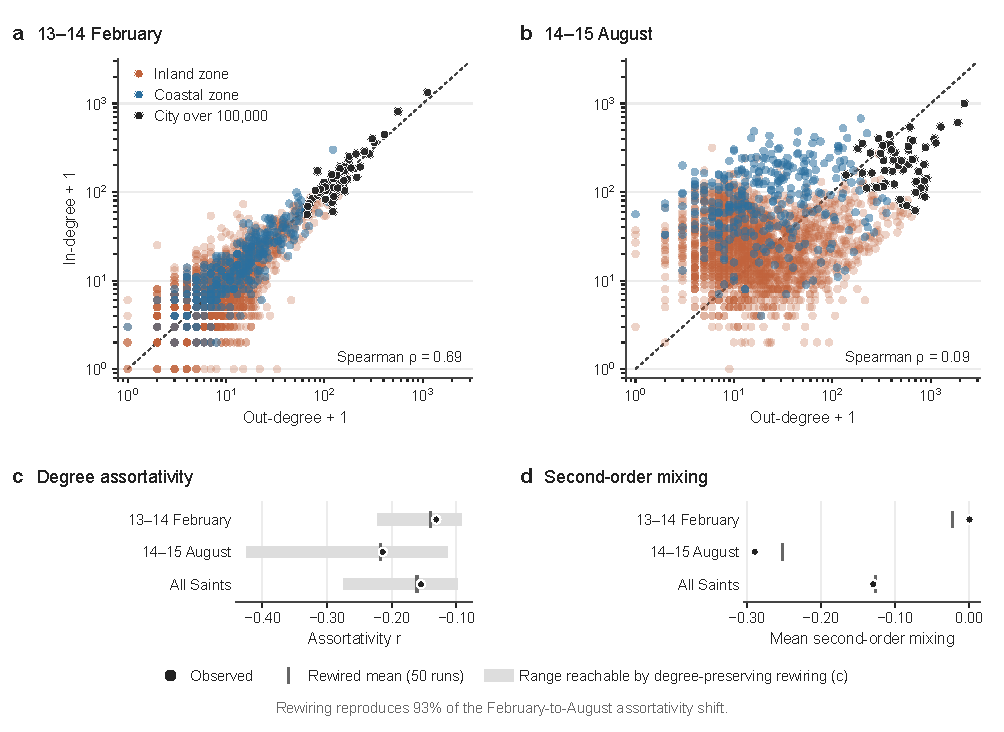
\includegraphics[width=\textwidth]{figS1.pdf}
\caption{\textbf{Holiday network structure against degree-preserving null models.} Ordinary night (13--14 February 2024), summer holiday (14--15 August) and All Saints (31 October--1 November). \textbf{a, b}, In-degree against out-degree of each zone, coloured by type (inland, coastal, city of more than 100,000 people). \textbf{c}, Degree assortativity: observed (point), mean of 50 degree-preserving rewirings (tick) and range reachable by rewiring while keeping degrees and connectivity (bar). \textbf{d}, Rich-club coefficient and second-order mixing against their null models. Links: at least 10 residents of $i$ sleeping in $j$.}
\label{fig:S1}
\end{figure}

For each main night I build a directed network on the 2,435 zones, with a link from $i$ to $j$ when at least ten residents of $i$ sleep in $j$. The summer network is about four times denser (undirected density 0.89\% on 13--14 February 2024, 3.44\% on 14--15 August). It splits into sending and receiving zones: the rank correlation of a zone's in- and out-degree falls from 0.69 to 0.09, and reciprocity from 0.52 to 0.24 (0.24 also when every night keeps the same number of directed links, 35,812). Degree assortativity falls from $-0.131$ to $-0.214$. Degree-preserving rewiring of the same networks gives $-0.140$ and $-0.217$: the null reproduces about 93\% of the change, so the summer network mixes the way its new degrees force it to \cite{maslov2002specificity,zhou2007structural}. The range of assortativity reachable by rewiring \cite{zhou2007structural} widens from $[-0.22,-0.09]$ to $[-0.42,-0.11]$. The rich-club coefficient of the 50 best-connected zones rises from 0.80 to 0.96, but its rewired value rises from 0.66 to 0.92, and the normalised coefficient falls from 1.22 to 1.05. The only property clearly beyond its null in summer is second-order mixing \cite{zhou2017second}, $-0.289$ against $-0.252$ under a null that keeps degrees and the rich-club profile. Two network-level claims explored earlier did not survive their nulls: the promotion of depopulated zones to the network core is reproduced by rewiring, and the communities of the bipartite city--zone network are more geographically compact than a calibrated gravity null, not less (non-contiguous share 71\% against 99\%).

The lesson for the main text is that the holiday network looks different on almost every structural measure because it is denser, as expected from the literature on comparing networks of different density \cite{vanwijk2010comparing,krings2012effects,cimini2019statistical}. The behavioural signal is in which links grow, which the roots elasticity measures directly.

%% ------------------------------------------------------------
\section{Robustness of the pre-registered tests}\label{si:robust}

\begin{figure}[t]
\centering
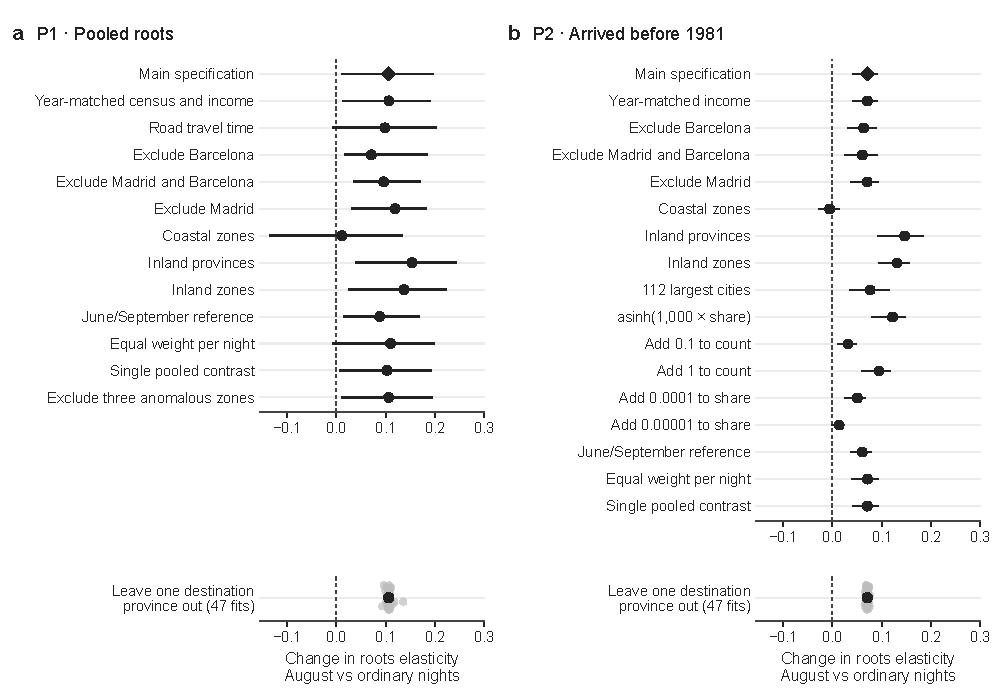
\includegraphics[width=\textwidth]{figS3.pdf}
\caption{\textbf{Robustness of the August contrasts, 2022--2024 confirmation.} \textbf{a}, P1 (all residents), P2 (arrived before 1981) and P3 (inland minus coast) under alternative specifications. \textbf{b}, Leave-one-destination-province-out estimates. 95\% wild cluster bootstrap intervals, clustered by origin province.}
\label{fig:S3}
\end{figure}

Table~\ref{tab:robust} lists the pre-registered robustness checks on the 2022--2024 confirmation. The pooled premium (P1) stays between 0.07 and 0.15; its interval touches zero when distance is measured by road travel time and when each night has equal weight. The pre-1981 term (P2) is positive with an interval above zero in every check except coastal destinations only. The inland-minus-coast difference (P3) is significant only with road travel time and vanishes when Madrid and Barcelona are dropped as origins.

\begin{table}[t]
\caption{\textbf{Robustness checks, 2022--2024 confirmation.} Estimate, 95\% wild cluster bootstrap interval and bootstrap $p$-value (not Holm-adjusted).}\label{tab:robust}
\footnotesize
\begin{tabular*}{\textwidth}{@{\extracolsep\fill}lccc}
\toprule
Check & P1 all residents & P2 arrived before 1981 & P3 inland $-$ coast \\
\midrule
Main specification & 0.106 [0.010, 0.197] & 0.071 [0.041, 0.092] & 0.122 [$-0.037$, 0.280] \\
Year-matched roots and income & 0.107 [0.013, 0.191] & 0.071 [0.041, 0.092] & --- \\
Road travel time & 0.099 [$-0.007$, 0.202] & --- & 0.152 [0.022, 0.347] \\
Drop Madrid origin & 0.119 [0.031, 0.183] & 0.071 [0.036, 0.093] & --- \\
Drop Barcelona origin & 0.071 [0.017, 0.185] & 0.064 [0.031, 0.089] & --- \\
Drop Madrid and Barcelona & 0.096 [0.035, 0.171] & 0.061 [0.024, 0.091] & 0.001 [$-0.126$, 0.244] \\
Inland zones only & 0.138 [0.024, 0.223] & 0.131 [0.093, 0.157] & --- \\
Inland provinces only (28) & 0.154 [0.039, 0.245] & 0.147 [0.091, 0.184] & --- \\
Coastal zones only & 0.011 [$-0.135$, 0.134] & $-0.005$ [$-0.028$, 0.014] & --- \\
Seasonal reference (June, September) & 0.088 [0.014, 0.168] & 0.060 [0.036, 0.080] & 0.079 [$-0.049$, 0.233] \\
Equal weight by night & 0.110 [$-0.007$, 0.200] & 0.071 [0.038, 0.093] & 0.132 [$-0.058$, 0.289] \\
Single pooled contrast across years & 0.103 [0.007, 0.193] & 0.071 [0.041, 0.093] & 0.128 [$-0.030$, 0.293] \\
\botrule
\end{tabular*}
\end{table}

%% ------------------------------------------------------------
\section{Sensitivity of the cohort results}\label{si:cohort}

\begin{figure}[t]
\centering
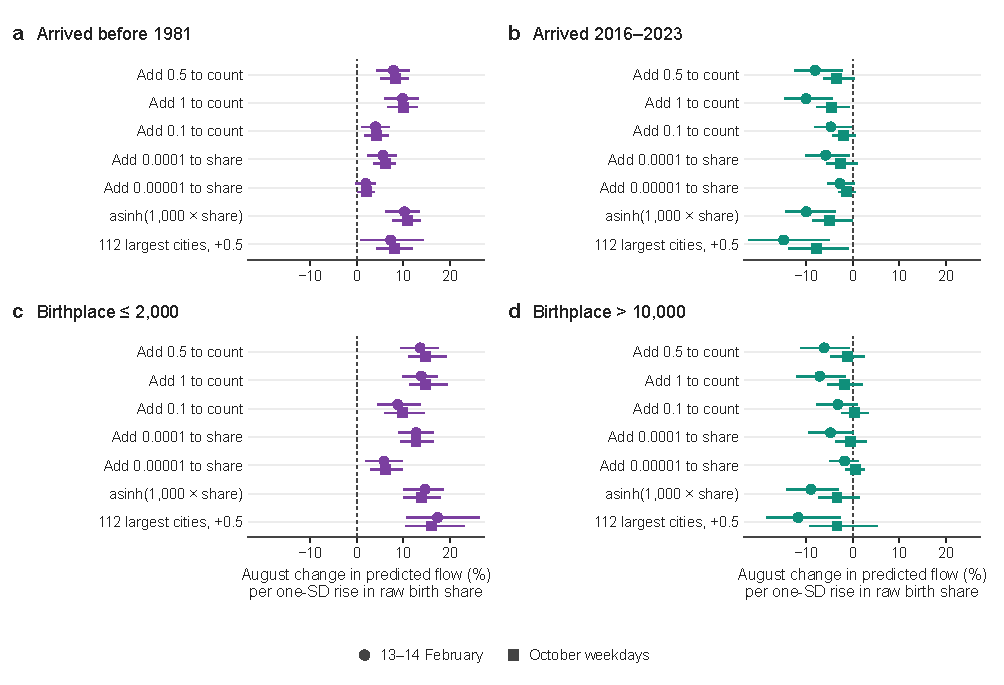
\includegraphics[width=\textwidth]{figS5.pdf}
\caption{\textbf{Cohort results under alternative rules for empty census cells.} August (14--15 August 2024) against 13--14 February 2024 and October 2024 weekdays, expressed as the percentage change in expected flow for a one-standard-deviation increase in the group share, so that rules are comparable. 95\% wild cluster bootstrap intervals, 44 origin-province clusters.}
\label{fig:S5}
\end{figure}

In a 10\% sample many city--province cells are empty for a group, so the log share needs a rule. The main text adds one half to each group count. Seven rules give the same sign for the pre-1981 and village-born terms; expressed as the percentage change in expected flow for a one-standard-deviation increase in the group share, six of them agree closely (pre-1981: $+4.1$\% to $+10.3$\% for all destinations, $+8.4$\% to $+14.9$\% inland; village-born: $+8.8$\% to $+17.4$\%). The exception, adding $10^{-5}$ to the share, gives extreme weight to pseudo-zeros and shrinks the pre-1981 effect to $+2.0$\% ($p=0.09$; inland $+5.2$\%, $p<0.001$). On the 2022--2024 confirmation the pre-1981 coefficient ranges from 0.014 to 0.122 across rules, so the sign is robust and the size approximate.

Further checks on the 2024 nights: (i) the special arrival codes of the census were dropped from both groups, which moves the estimates by at most 0.0016; (ii) within age bands, residents who arrived before 1981 gain more than later arrivals among those aged 65 and over ($+0.095$ against February, $+0.057$ against October) and among those aged 43--64 ($+0.040$, $+0.034$); (iii) the results hold when each of the 44 origin provinces and each of the 47 destination provinces is left out, and when Madrid and Barcelona are dropped together (42 clusters); (iv) the pre-1981 and village-born terms keep their sign in all 117 pairs of an August-window night and a February weekday night of 2024 and in 108 pairs built with October 2024, 2022 and 2023. These pairs share nights and cities and are not independent replications. The recent-arrival decline is $-0.071$ against February but $-0.029$ ($p=0.08$) against October, because February has an unusually high recent-arrival slope; the difference between pre-1981 and recent arrivals is positive against both ($+0.155$ and $+0.116$).

%% ------------------------------------------------------------
\section{The receiving end}\label{si:receiving}

\begin{table}[t]
\caption{\textbf{Most depopulated fifth of zones: share of net receivers by type of night, 2022--2024.} 475 zones; ordinary nights by month (monthly means and range).}\label{tab:receiving}
\footnotesize
\begin{tabular*}{\textwidth}{@{\extracolsep\fill}lccc}
\toprule
Nights & Nights (n) & Mean share & Range \\
\midrule
Ordinary, January--March & 93 & 0.38--0.39$^{a}$ & 0.18--0.69 \\
Ordinary, April--June & 85 & 0.72--0.81$^{a}$ & 0.52--0.88 \\
Ordinary, September & 22 & 0.74 & 0.63--0.85 \\
Ordinary, October & 28 & 0.49 & 0.35--0.65 \\
Ordinary, November--December & 52 & 0.27--0.28$^{a}$ & 0.17--0.50 \\
August window (10--18 August) & 27 & 0.98 & 0.97--0.99 \\
\botrule
\end{tabular*}
\footnotetext{$^{a}$ Range of the monthly means within the period.}
\end{table}

Table~\ref{tab:receiving} gives the seasonal cycle. On 14--15 August 2024 these zones received 0.71 visitors per resident (0.07 on 13--14 February) and sent 0.08 residents per resident elsewhere (0.10 in February); on Christmas Eve 0.38 and 0.14. Relative to the least depopulated fifth, about three quarters of the August gap comes from arrivals and one quarter from fewer departures, because departures from the least depopulated zones triple in August. In a model on inland zones with controls for population, number of municipalities, area, distance to the coast and to the nearest city, and province, the August change relative to February is $+0.144$ arrivals per resident (95\% CI 0.058--0.224) and $-0.076$ departures ($-0.090$ to $-0.060$), close to Christmas Eve ($+0.120$ and $-0.080$). With all zones, coastal resorts with very large August arrivals dominate the arrival term and the controlled August arrivals coefficient is not detected ($-0.040$).

\paragraph{Second homes.} Adding the share of non-primary dwellings (Census 2021 \cite{ine2023viviendas}) to the regression of the log change in visitors on the depopulation rank reduces the rank coefficient by 48\% in August and 2\% on Christmas Eve (paired difference 0.209, 95\% CI 0.120--0.292 by zone bootstrap). This is an attenuation of a coefficient, not a mediation analysis, and it is not detected in single-municipality zones alone (0.083, $-0.039$ to 0.184). I therefore do not draw conclusions about where visitors sleep.

%% ------------------------------------------------------------
\section{Parents' villages}\label{si:parents}

\begin{figure}[t]
\centering
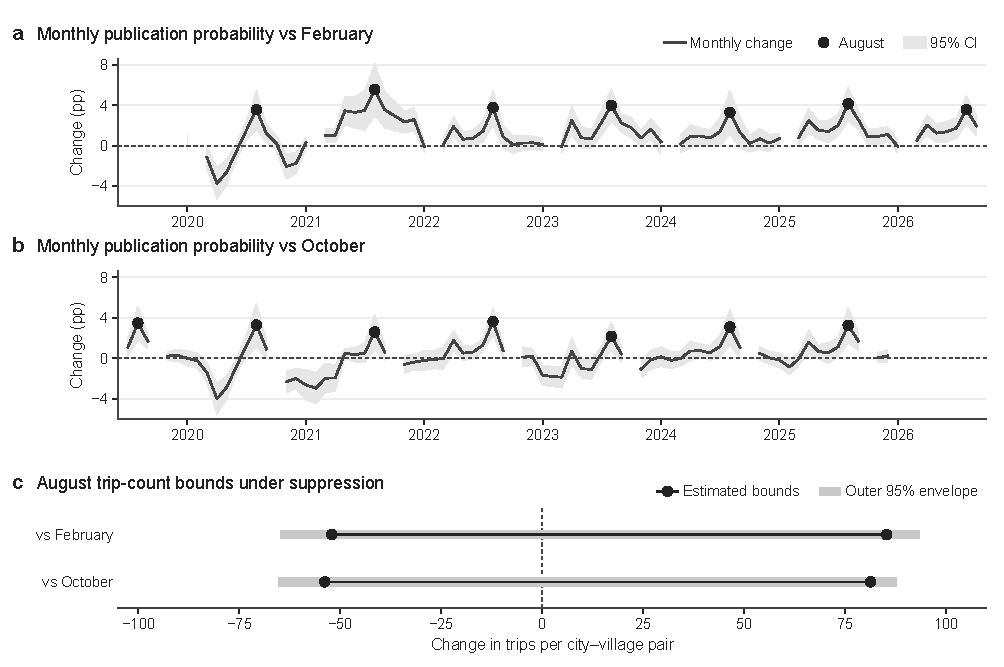
\includegraphics[width=\textwidth]{figS2.pdf}
\caption{\textbf{Flows to the villages where residents' parents were born.} 137 cities $\times$ 5,849 mainland municipalities of up to 2,000 inhabitants in other provinces. \textbf{a}, Change in the probability that the city-to-village flow appears in the published municipal trip matrices, for pairs with a parental tie, by month against February and October of the same year. \textbf{b}, Change in trips under alternative treatments of withheld cells (set to 0, set to 29, and the interval between them). 95\% intervals combine two-way province clustering and 399 survey resamples.}
\label{fig:S2}
\end{figure}

The national survey ECEPOV 2021 \cite{ine2023ecepovmicro} records the exact birth municipality of each respondent and of both parents. For city-born respondents in the 137 cities, I counted, for each city and each mainland municipality of up to 2,000 inhabitants in another province, the survey-weighted share of parent birthplaces in that village (7,988 city--village pairs have a parental tie). The outcome is the monthly number of trips from city to village in the statistics office's three-operator matrices \cite{ine2026turismomoviles}, July 2019 to September 2026, which withhold flows below 30 trips. Municipal geometry comes from Eurostat \cite{gisco2021lau}. The design compares villages of the same province receiving visitors from the same city, with city~$\times$~province and village effects.

Pre-registered gate (Section~\ref{si:prereg}): (1) the August change in publication probability must be positive against February and October; (2) the change in trips must be positive under at least two treatments of the withheld cells; (3) intervals must propagate survey uncertainty and cluster in both province dimensions; (4) real municipal geometry must be used. Conditions 1, 3 and 4 pass: a parental tie raises the August-minus-February probability of publication by 4.0 percentage points (95\% CI 2.2--5.7) and the August-minus-October probability by 3.1 (1.5--4.6), with a dose response in the strength of the tie. Condition 2 fails. Setting withheld cells to 0 or to 29 gives positive changes ($+17$ and $+16$ trips against February), but these are two scenarios of the same method; allowing each withheld cell to take any value between 0 and 29 gives a confidence envelope from $-65$ to $+93$ trips, and on the 360 pairs published every month the change is $-0.16$ log points ($-0.83$ to 0.51). The analysis therefore stays here as a limit of the published data: flows towards parents' villages cross the publication threshold more often in August, but the data cannot say by how many trips they grow.

%% ------------------------------------------------------------
\section{The July 2025 change of method}\label{si:bridge}

\begin{figure}[t]
\centering
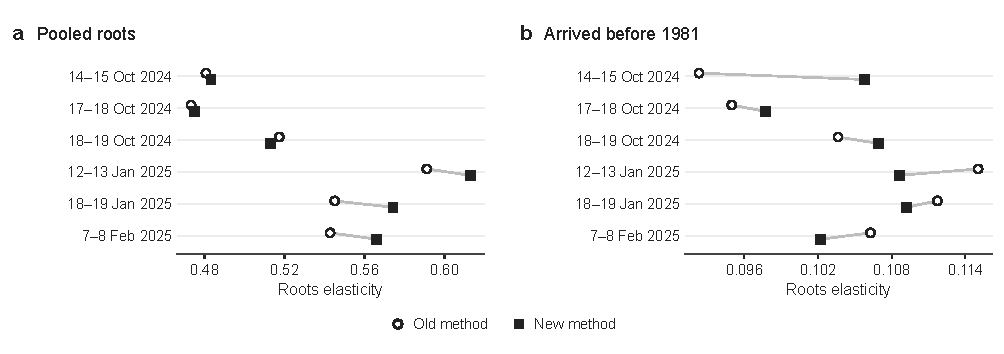
\includegraphics[width=0.7\textwidth]{figS4.pdf}
\caption{\textbf{Method bridge.} Roots elasticity (all residents) and pre-1981 term on the six dates the ministry computed with both methods.}
\label{fig:S4}
\end{figure}

On 1 July 2025 the ministry changed its filter for static devices on road networks \cite{mitms2025methodchange} and recalculated six dates with the new method. On these dates the new method raises the mainland total away from home by 4--6\% and lowers the overall total by under 1\%. The roots elasticity changes by $+0.003$, $+0.002$, $-0.005$, $+0.022$, $+0.029$ and $+0.023$ (mean absolute change 0.014; registered tolerance 0.035), and the pre-1981 term by at most 0.014 (mean absolute change 0.005; tolerance 0.024). The bridge passed, so the 2025 hold-out compares the five August nights (new method) with ordinary nights of January--June (old method) and October 2025 (new method).

%% ------------------------------------------------------------
\section{Pre-registration and deviations}\label{si:prereg}

The pre-registration (\texttt{journal/analysis/PREREGISTRATION.md} and \texttt{design.yml} in the repository) was committed on 27 November 2026 before the 779 new nights of 2022--2024 were opened. It fixed the night classes and quality rules, the two models, the primary hypotheses (P1--P3), the secondary hypotheses (S1--S6), the inference and the Holm families, the decision rule and the gate for the parents'-village analysis. Two deviations were recorded:
\begin{enumerate}
\item \emph{No new August nights in the 2022--2024 confirmation.} Every August night of 2022--2024 had been in the earlier cache, so that confirmation compares seen August nights with new ordinary nights. A second confirmation on 2025 was registered before any 2025 file was downloaded, with the method bridge of Section~\ref{si:bridge}.
\item \emph{Three zones with data drop-outs} were meant to be excluded and were kept as destinations in the 2022--2024 estimates. Excluding them changes the 2025 estimates by at most 0.0005 and no Holm decision.
\end{enumerate}
Analyses added after the registration and labelled as such: the split of the confirmation into strictly unseen nights, the descriptive calendar summaries, and the seasonal breakdown of the receiving end.

\bibliography{references}

\end{document}
